\chapter{Ярость к конечным автоматам}
\label{rage-against-the-finite-state-machines}
\section{Кто они такие?}
\label{what-are-they}
Конечные автоматы (КА) не имеют ничего общего с огнестрельным оружием.
Их главным признаком является наличие конечного числа состояний.
Мне всегда было проще понимать конечные автоматы, если они изображены в виде графиков и диаграмм.
К примеру, такая нехитрая диаграмма описывает (очень глупую) собаку в виде автомата состояний.
\begin{figure}[h!]
    \centering
    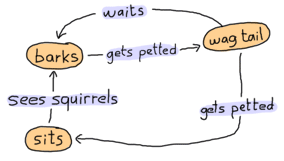
\includegraphics[width=0.7\textwidth]{fsm_dog.png}
\end{figure}
Собака может находиться в трёх состояниях: она может сидеть, гавкать или вилять хвостом.
Различные события или входящие данные могут вынудить её поменять состояние.
Если собака спокойно сидит и замечает белку, она начнёт гавкать и будет продолжать гавкать, пока её не погладят.
Но если собака сидит и вы её погладите, мы даже не можем вообразить, что может произойти.
В мире Erlang собака могла бы аварийно завершиться (и со временем её перезапустил бы супервизор).
В реальности такое событие бы выглядело пугающе: ваша собака, после того как её задавила машина, просто вернулась бы домой, что в целом не так уж и плохо.

Для сравнения я приведу диаграмму состояний кошки:

\begin{figure}[h!]
    \centering
    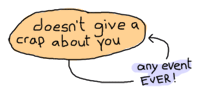
\includegraphics[width=0.7\textwidth]{fsm_cat.png}
\end{figure}

Эта кошка всегда находится в одном и том же состоянии, и никакое событие не сможет его изменить.

\href{http://learnyousomeerlang.com/static/erlang/cat\_fsm.erl}{Автомат, который описывает состояния кошки}, можно легко и просто реализовать на Erlang:
\begin{lstlisting}[style=erlang]
-module(cat_fsm).
-export([start/0, event/2]).
 
start() ->
    spawn(fun() -> dont_give_crap() end).
 
event(Pid, Event) ->
    Ref = make_ref(), % won't care for monitors here
    Pid ! {self(), Ref, Event},
    receive
        {Ref, Msg} -> {ok, Msg}
    after 5000 ->
        {error, timeout}
    end.
 
dont_give_crap() ->
    receive
        {Pid, Ref, _Msg} -> Pid ! {Ref, meh};
        _ -> ok
    end,
    io:format("Switching to 'dont_give_crap' state~n"),
    dont_give_crap().
\end{lstlisting}
Мы можем воспользоваться модулем, чтобы убедиться, что кошка действительно всегда сохраняет невозмутимость:
\begin{lstlisting}[style=erlang]
1> c(cat_fsm).
{ok,cat_fsm}
2> Cat = cat_fsm:start().
<0.67.0>
3> cat_fsm:event(Cat, pet).
Switching to 'dont_give_crap' state
{ok,meh}
4> cat_fsm:event(Cat, love).
Switching to 'dont_give_crap' state
{ok,meh}
5> cat_fsm:event(Cat, cherish).
Switching to 'dont_give_crap' state
{ok,meh}
\end{lstlisting}
То же самое можно сделать и для \href{http://learnyousomeerlang.com/static/erlang/dog\_fsm.erl}{конечного автомата, который описывает поведение собаки}.
В отличие от кошки, собаке доступно большее количество состояний:
\begin{lstlisting}[style=erlang]
-module(dog_fsm).
-export([start/0, squirrel/1, pet/1]).
 
start() ->
    spawn(fun() -> bark() end).
 
squirrel(Pid) -> Pid ! squirrel.
 
pet(Pid) -> Pid ! pet.
 
bark() ->
    io:format("Dog says: BARK! BARK!~n"),
    receive
        pet ->
            wag_tail();
        _ ->
            io:format("Dog is confused~n"),
            bark()
    after 2000 ->
        bark()
    end.
 
wag_tail() ->
    io:format("Dog wags its tail~n"),
    receive
        pet ->
            sit();
        _ ->
            io:format("Dog is confused~n"),
            wag_tail()
    after 30000 ->
        bark()
    end.
 
sit() ->
    io:format("Dog is sitting. Gooooood boy!~n"),
    receive
        squirrel ->
            bark();
        _ ->
            io:format("Dog is confused~n"),
            sit()
    end.
\end{lstlisting}
Мы сможем относительно легко установить соответствие каждого состояния и перехода с тем, что было изображено на диаграмме.
Вот как выглядит конечный автомат в деле:
\begin{lstlisting}[style=erlang]
6> c(dog_fsm).
{ok,dog_fsm}
7> Pid = dog_fsm:start().
Dog says: BARK! BARK!
<0.46.0>
Dog says: BARK! BARK!
Dog says: BARK! BARK!
Dog says: BARK! BARK!
8> dog_fsm:pet(Pid).
pet
Dog wags its tail
9> dog_fsm:pet(Pid).
Dog is sitting. Gooooood boy!
pet
10> dog_fsm:pet(Pid).
Dog is confused
pet
Dog is sitting. Gooooood boy!
11> dog_fsm:squirrel(Pid).
Dog says: BARK! BARK!
squirrel
Dog says: BARK! BARK!   
12> dog_fsm:pet(Pid).
Dog wags its tail
pet
13> %% wait 30 seconds
Dog says: BARK! BARK!
Dog says: BARK! BARK!
Dog says: BARK! BARK!    
13> dog_fsm:pet(Pid).    
Dog wags its tail
pet
14> dog_fsm:pet(Pid).
Dog is sitting. Gooooood boy!
pet
\end{lstlisting}

Можете, если хотите, отслеживать состояния по схеме (я обычно так и делаю \--- это помогает убедиться, что мы нигде не ошиблись).

Вот, собственно, основа конечного автомата, реализованного при помощи процессов Erlang.
Мы могли бы кое\--что сделать иначе: можно было бы передавать состояние в аргументах функций состояния, подобно тому как мы это делаем в реализации главного серверного цикла.
Также мы могли бы добавить функции \ops{init} и \ops{terminate}, обработку обновления кода и т.п.

Есть и ещё одно отличие между конечными автоматами собаки и кошки \--- кошка использует \emph{синхронные} события, а собака \emph{асинхронные}.
В реальном конечном автомате можно было бы использовать и тот и другой вид событий, но из\--за чистой незамутнённой лени, я выбрал самое простое представление из возможных.
Также существует ещё один вид событий, не показанный в примерах \--- глобальные события, которые могут возникать в любом состоянии.

Примером такого события может стать ситуация, когда собака учуяла еду.
Как только сработает событие \ops{smell\_food}, пёс начнёт искать источник запаха, в каком бы состоянии он ни находился. 

Но не будем долго задерживаться на реализации всего перечисленного в нашем грубом наброске конечного автомата.
Лучше перейдём прямо к стратегии поведения \ops{gen\_fsm}.
\section{Обобщённые конечные автоматы}
\label{generic-finite-state-machines}
Стратегия поведения \ops{gen\_fsm} схожа с \ops{gen\_server} тем, что она является её специализированной разновидностью.
Главное отличие gen\_fsm заключается в том, что вместо обработки \emph{вызовов (calls)} и \emph{cast-запросов (casts)} мы обрабатываем \emph{синхронные} и \emph{асинхронные события}.
Каждое состояние, как и в наших примерах с кошкой и собакой, представлено функцией.
Мы снова перечислим функции обратного вызова, которые должны быть реализованы нашими модулями для корректной работы.
\subsection{init}
\label{init2}
Это тот же самый \href{http://erldocs.com/R15B/stdlib/gen\_fsm.html\#init/1}{init/1}, который используется в серверах общего назначения, но с несколькими отличиями: он допускает в качестве возвращаемых значений кортежи \ops{\{ok, StateName, Data\}}, \ops{\{ok, StateName, Data, Timeout\}}, \ops{\{ok, StateName, Data, hibernate\}} и \ops{\{stop, Reason\}}.
Кортеж с атомом \ops{stop} работает так же как в \ops{gen\_server}\--ах, а для \ops{hibernate} с \emph{Timeout} сохраняется та же семантика.

Новизна скрывается в переменной \emph{StateName}.
\emph{StateName} это атом, определяющий функцию обратного вызова, которую необходимо вызвать следующей.
\subsection{StateName}
\label{statename}
\begin{wrapfigure}{r}{0.35\linewidth}
    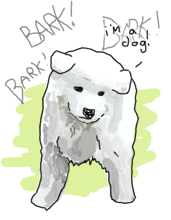
\includegraphics[width=1\linewidth]{dog.png}
\end{wrapfigure}
Функции \href{http://erldocs.com/R15B/stdlib/gen\_fsm.html\#StateName/2}{StateName/2} и \href{http://erldocs.com/R15B/stdlib/gen\_fsm.html\#StateName/2}{StateName/3} носят имена\--заполнители (placeholders), и именно вы должны заменить их теми именами, которые посчитаете нужными.
Предположим, что функция \ops{init/1} возвращает кортеж \ops{\{ok, sitting, dog\}}.
Значит, конечный автомат находится в состоянии \ops{sitting}.
Это не та же разновидность состояния, которую мы видели в \ops{gen\_server}, она скорее служит эквивалентом для состояний \ops{sit}, \ops{bark} и \ops{wag\_tail} предыдущего конечного автомата, описывающего поведение собаки.
Эти состояния задают контекст, в котором вы обрабатываете заданное событие.

Как пример можно привести ситуацию, когда кто\--либо звонит вам по телефону.
Если ваше текущее состояние <<утренний субботний сон>, то на звонок вы, должно быть, отреагируете криками в телефонную трубку.
Если ваше состояние <<ожидаю собеседования>>, то вы, скорее всего, вежливо ответите на звонок.
Ну и если вы пребываете в состоянии <<умер>>, то мне не вполне ясно как вы вообще смогли прочитать эти строки.

Вернёмся к нашему конечному автомату.
Функция \ops{init/1} сообщила, что мы должны находиться в состоянии \ops{sitting}.
Всякий раз когда процесс \ops{gen\_fsm} принимает уведомление о событии, будет вызвана либо функция \ops{sitting/2}, либо \ops{sitting/3}.
Функция \ops{sitting/2} вызывается для асинхронных событий, а \ops{sitting/3} для синхронных.

Аргументами для \ops{sitting/3} будут \emph{Event}, само сообщение, переданное в качестве события, и \emph{StateData}: данные, которые переносились от вызова к вызову.
Затем функция \ops{sitting/2} сможет возвратить кортежи \ops{\{next\_state, NextStateName, NewStateData\}}, \ops{\{next\_state, NextStateName, NewStateData, Timeout\}}, \ops{\{next\_state, NextStateName, hibernate\}} и \ops{\{stop, Reason, NewStateData\}}.

Для \ops{sitting/3} задаются схожие аргументы, только между \emph{Event} и \emph{StateData} передаётся еще и переменная \emph{From}.
Переменная \emph{From} используется совершенно так же как она использовалась в \ops{gen\_server}\--ах, включая \href{http://erldocs.com/R15B/stdlib/gen\_fsm.html\#reply/2}{gen\_fsm:reply/2}.
Функции \ops{StateName/3} могут возвращать следующие кортежи:
\begin{lstlisting}[style=erlang]
{reply, Reply, NextStateName, NewStateData}
{reply, Reply, NextStateName, NewStateData, Timeout}
{reply, Reply, NextStateName, NewStateData, hibernate}

{next_state, NextStateName, NewStateData}
{next_state, NextStateName, NewStateData, Timeout}
{next_state, NextStateName, NewStateData, hibernate}

{stop, Reason, Reply, NewStateData}
{stop, Reason, NewStateData}
\end{lstlisting}

Заметьте, что количество этих функций никак не ограничивается, но лишь при условии, что они проэкспортированы.
Атомы, возвращаемые в кортежах как \emph{NextStateName}, определяют, будет ли функция вызвана или нет.

\subsection{handle\_event}
\label{handle-event}
В предыдущем разделе я упомянул о глобальных событиях, которые могут спровоцировать определённую реакцию, не зависящую от нашего текущего состояния (собака, которая учуяла пищу, бросит своё текущее занятие, и приступит к поиску еды).
Для событий, которые необходимо обрабатывать одинаково в каждом состоянии, лучше всего подойдёт функция обратного вызова (callback) \href{http://erldocs.com/R15B/stdlib/gen\_fsm.html\#handle\_event/3}{handle\_event/3}.
Список аргументов для этой функции похож на \ops{StateName/2}, за исключением дополнительной переменной \emph{StateName}, которая указывает, каким было состояние в момент получения события.
Возвращает она те же значения, что и \ops{StateName/2}.
\subsection{handle\_sync\_event}
\label{handle-sync-event}
Функция обратного вызова \href{http://erldocs.com/R15B/stdlib/gen\_fsm.html\#handle\_sync\_event/4}{handle\_sync\_event/4} относится к \ops{StateName/3} так же, как \ops{handle\_event/2} относится к \ops{StateName/2}.
Она обрабатывает синхронные глобальные события, принимает те же самые параметры и возвращает кортежи того же вида, что и \ops{StateName/3}.

Настал подходящий момент для объяснения принципа, по которому мы определяем, относиться ли событие к глобальным, или его необходимо обрабатывать в определённом состоянии.
Для этого мы можем взглянуть на функцию, которая используется для отсылки события к КА (конечному автомату).
Асинхронные события, предназначенные для любой функции \ops{StateName/2} отправляются при помощи \href{http://erldocs.com/R15B/stdlib/gen\_fsm.html\#send\_event/2}{send\_event/2}, а синхронные события, которые должны обрабатываться \ops{StateName/3} отсылаются \href{http://erldocs.com/R15B/stdlib/gen\_fsm.html\#sync\_send\_event/2}{sync\_send\_event/2-3}.

Для глобальных событий двумя эквивалентными функциями являются \href{http://erldocs.com/R15B/stdlib/gen\_fsm.html\#send\_all\_state\_event/2}{send\_all\_state\_event/2} и \href{http://erldocs.com/R15B/stdlib/gen\_fsm.html\#sync\_send\_all\_state\_event/2}{sync\_send\_all\_state\_event/2-3} (весьма длинное имя).

\subsection{code\_change}
\label{code-change}
Эта функция выполняется совершенно так же, как и для \ops{gen\_server}\--а, за исключением того, что она принимает дополнительный параметр состояния, когда её вызов выглядит как \ops{code\_change(OldVersion, StateName, Data, Extra)}, и возвращает кортеж вида \ops{\{ok, NextStateName, NewStateData\}}.

\subsection{terminate}
\label{terminate}
Эта функция, опять же, действует приблизительно так же, как и для обобщенных серверов.
Функция \href{http://erldocs.com/R15B/stdlib/gen\_fsm.html\#terminate/3}{terminate/3} должна выполнять действия, противоположные тем, которые выполняются в \ops{init/1}.

\section{Спецификация торговой системы}
\label{a-trading-system-specification}

Пора найти применение изученному материалу.
Многие руководства по Erlang, которые рассказывают о конечных автоматах, используют примеры, содержащие телефонные коммутаторы и тому подобные вещи.
Я рискну предположить, что большинство программистов будут редко сталкиваться с телефонными коммутаторами в контексте конечных автоматов.
Поэтому мы рассмотрим пример более подходящий для многих разработчиков: мы спроектируем и реализуем торговую систему для некоторой вымышленной и несуществующей видеоигры.

Я выбрал немного усложнённую схему для нашей системы.
Вместо того, чтобы использовать брокер, через которого игроки направляют товары и подтверждения (что, по правде говоря, было бы проще), мы реализуем сервер, при помощи которого оба игрока общаюся между собой напрямую (что даёт преимущество в виде распределённости системы).

Из\--за нетривиальности реализации, я довольно много времени потрачу на её описание, на рассмотрение задач, с которыми мы столкнемся и путями их решения.

Прежде всего мы должны определить действия, которые могут выполняться нашими игроками при торговле.
Первым действием будет запрос на открытие торговли.
Пользователь\--партнёр должен иметь возможность одобрить начало торговли.
Мы, впрочем, не будем давать им право отклонить торговую операцию, так как излишнее усложнение системы нам не нужно.
Эту функцию проще добавить после завершения всего проекта.

Как только торговая операция открыта, наши пользователи должны иметь возможность вести друг с другом переговоры.
Это означает, что они должны иметь возможность делать предложения, и при желании их отзывать.
Когда оба игрока удовлетворены предложением, каждый из них может заявить о своей готовности довести сделку до конца.
После этого данные об операции должны быть каким\--либо образом сохранены у обеих сторон.
В любой момент времени для любого из игроков должна быть возможность полностью отменить торговую операцию.
Какой\--нибудь \emph{плебей}, возможно, будет предлагать лишь  товары, которые не подобают величию противоположной стороны (которая может быть очень занята), и поэтому следует иметь возможность достойно ответить ему вполне заслуженным отказом.

Вкратце, наша система будет разрешать следующие действия:
\begin{itemize}
    \item запросить начало торговой  операции
    \item одобрить торговую операцию
    \item предложить предметы торговли
    \item отозвать предложение
    \item заявить о готовности довести сделку до конца
    \item резко отменить торговую операцию
\end{itemize}
А теперь, когда произведено каждое из этих действий, необходимо об этом уведомить конечный автомат второго игрока.
В этом действии есть смысл, ведь когда Джим приказывает своему конечному автомату отправить некоторый элемент Карлу, то конечный автомат Карла должен быть поставлен об этом в известность.
А значит оба игрока могут обращаться к собственным конечным автоматам, которые будут, в свою очередь, общаться с другими конечными автоматами.
Описанная схема будет выглядеть приблизительно так:

\begin{figure}[h!]
    \centering
    \includegraphics[width=0.7\textwidth]{fsm\_talk.png}
\end{figure}

Первое, что бросается в глаза: когда два идентичных процесса общаются друг с другом, необходимо держаться подальше от синхронных вызовов.
Делать это нужно потому, что если конечный автомат Джима посылает сообщение конечному автомату Карла, а затем ожидает ответа, в то самое время когда конечный автомат Карла посылает сообщение конечному автомату Джима и ожидает определенное ответное сообщение, то обе стороны будут ожидать ответа, сами при этом ответ никогда не отошлют.
Такая ситуация фактически замораживает оба конечных автомата.
То есть мы получаем взаимную блокировку процессов (deadlock).

Одним из решений этой ситуации было бы ожидание таймаута и продолжение исполнения кода, но тогда в обоих почтовых ящиках процессов остались бы необработанные сообщения, и протокол взаимодействия был бы нарушен.
Это, естественно, порождает целый клубок проблем, которого нам хотелось бы избежать.
Проще всего решить эту проблему отказом от синхронных сообщений и полностью перейти на асинхронное взаимодействие.
Обратите внимание, что Джим сможет делать синхронные запросы к собственному конечному автомату.
Риска в этом никакого нет, так как конечному автомату нет нужды вызывать Джима, и между ними взаимная блокировка возникнуть не может.

Когда оба этих конечных автомата общаются между собой, их обмен сообщениями может выглядеть как-то так:

\begin{figure}[h!]
    \centering
    \includegraphics[width=0.7\textwidth]{fsm\_overview.png}
\end{figure}

Оба конечных автомата находятся в состоянии бездействия.
Когда вы просите Джима начать торговлю, Джим должен принять предложение, прежде чем двигаться дальше.
Затем вы оба сможете предлагать товары или снимать их с торга.
Когда оба участника объявили о своей готовности, может начаться торговля.
Так выглядит упрощенная версия возможных событий, и о всех возможных случаях мы поговорим подробнее в следующих параграфах.

А теперь сложный момент: как определить диаграмму состояний, и как будут происходить переходы между этими состояниями.
Как правило, обдумывание этого вопроса занимает много времени, так как вам необходимо учесть любую, даже самую малую возможность того, что что-то пойдет не так.
Что-то может пойти не так даже после многократного рассмотрения всех нюансов.
Поэтому я просто приведу здесь диаграму, которую я решил реализовать, а затем прокомментирую ее.

\begin{figure}[h!]
    \centering
    \includegraphics[width=0.7\textwidth]{fsm\_general.png}
\end{figure}

Сначала оба конечных автомата стартуют в состоянии \ops{idle}.
В этот момент единственное, что мы можем сделать \--- попросить другого игрока вести с нами переговоры:

\begin{figure}[h!]
    \centering
    \includegraphics[width=0.7\textwidth]{fsm\_initiate\_nego.png}
\end{figure}

Мы переходим в режим \ops{idle\_wait}, чтобы ожидать ответ на запрос нашего конечного автомата.
Как только другой автомат вышлет ответ, наш может переключиться в режим \ops{negotiate}:

\begin{figure}[h!]
    \centering
    \includegraphics[width=0.7\textwidth]{fsm\_other\_accept.png}
\end{figure}

После этого шага противоположная сторона также будет находиться в состоянии \ops{negotiate}.
Само собой разумеется, что если мы можем пригласить другого игрока, то и он тоже может пригласить нас.
Если все пройдет нормально, взаимодействие будет выглядеть так:

\begin{figure}[h!]
    \centering
    \includegraphics[width=0.7\textwidth]{fsm\_other\_initiate\_nego.png}
\end{figure}
